Résumons rapidement la méthode d'estimation de la régularité en un point $t_2 \in \mathcal T$.

\begin{figure}[H]
	\begin{center}
		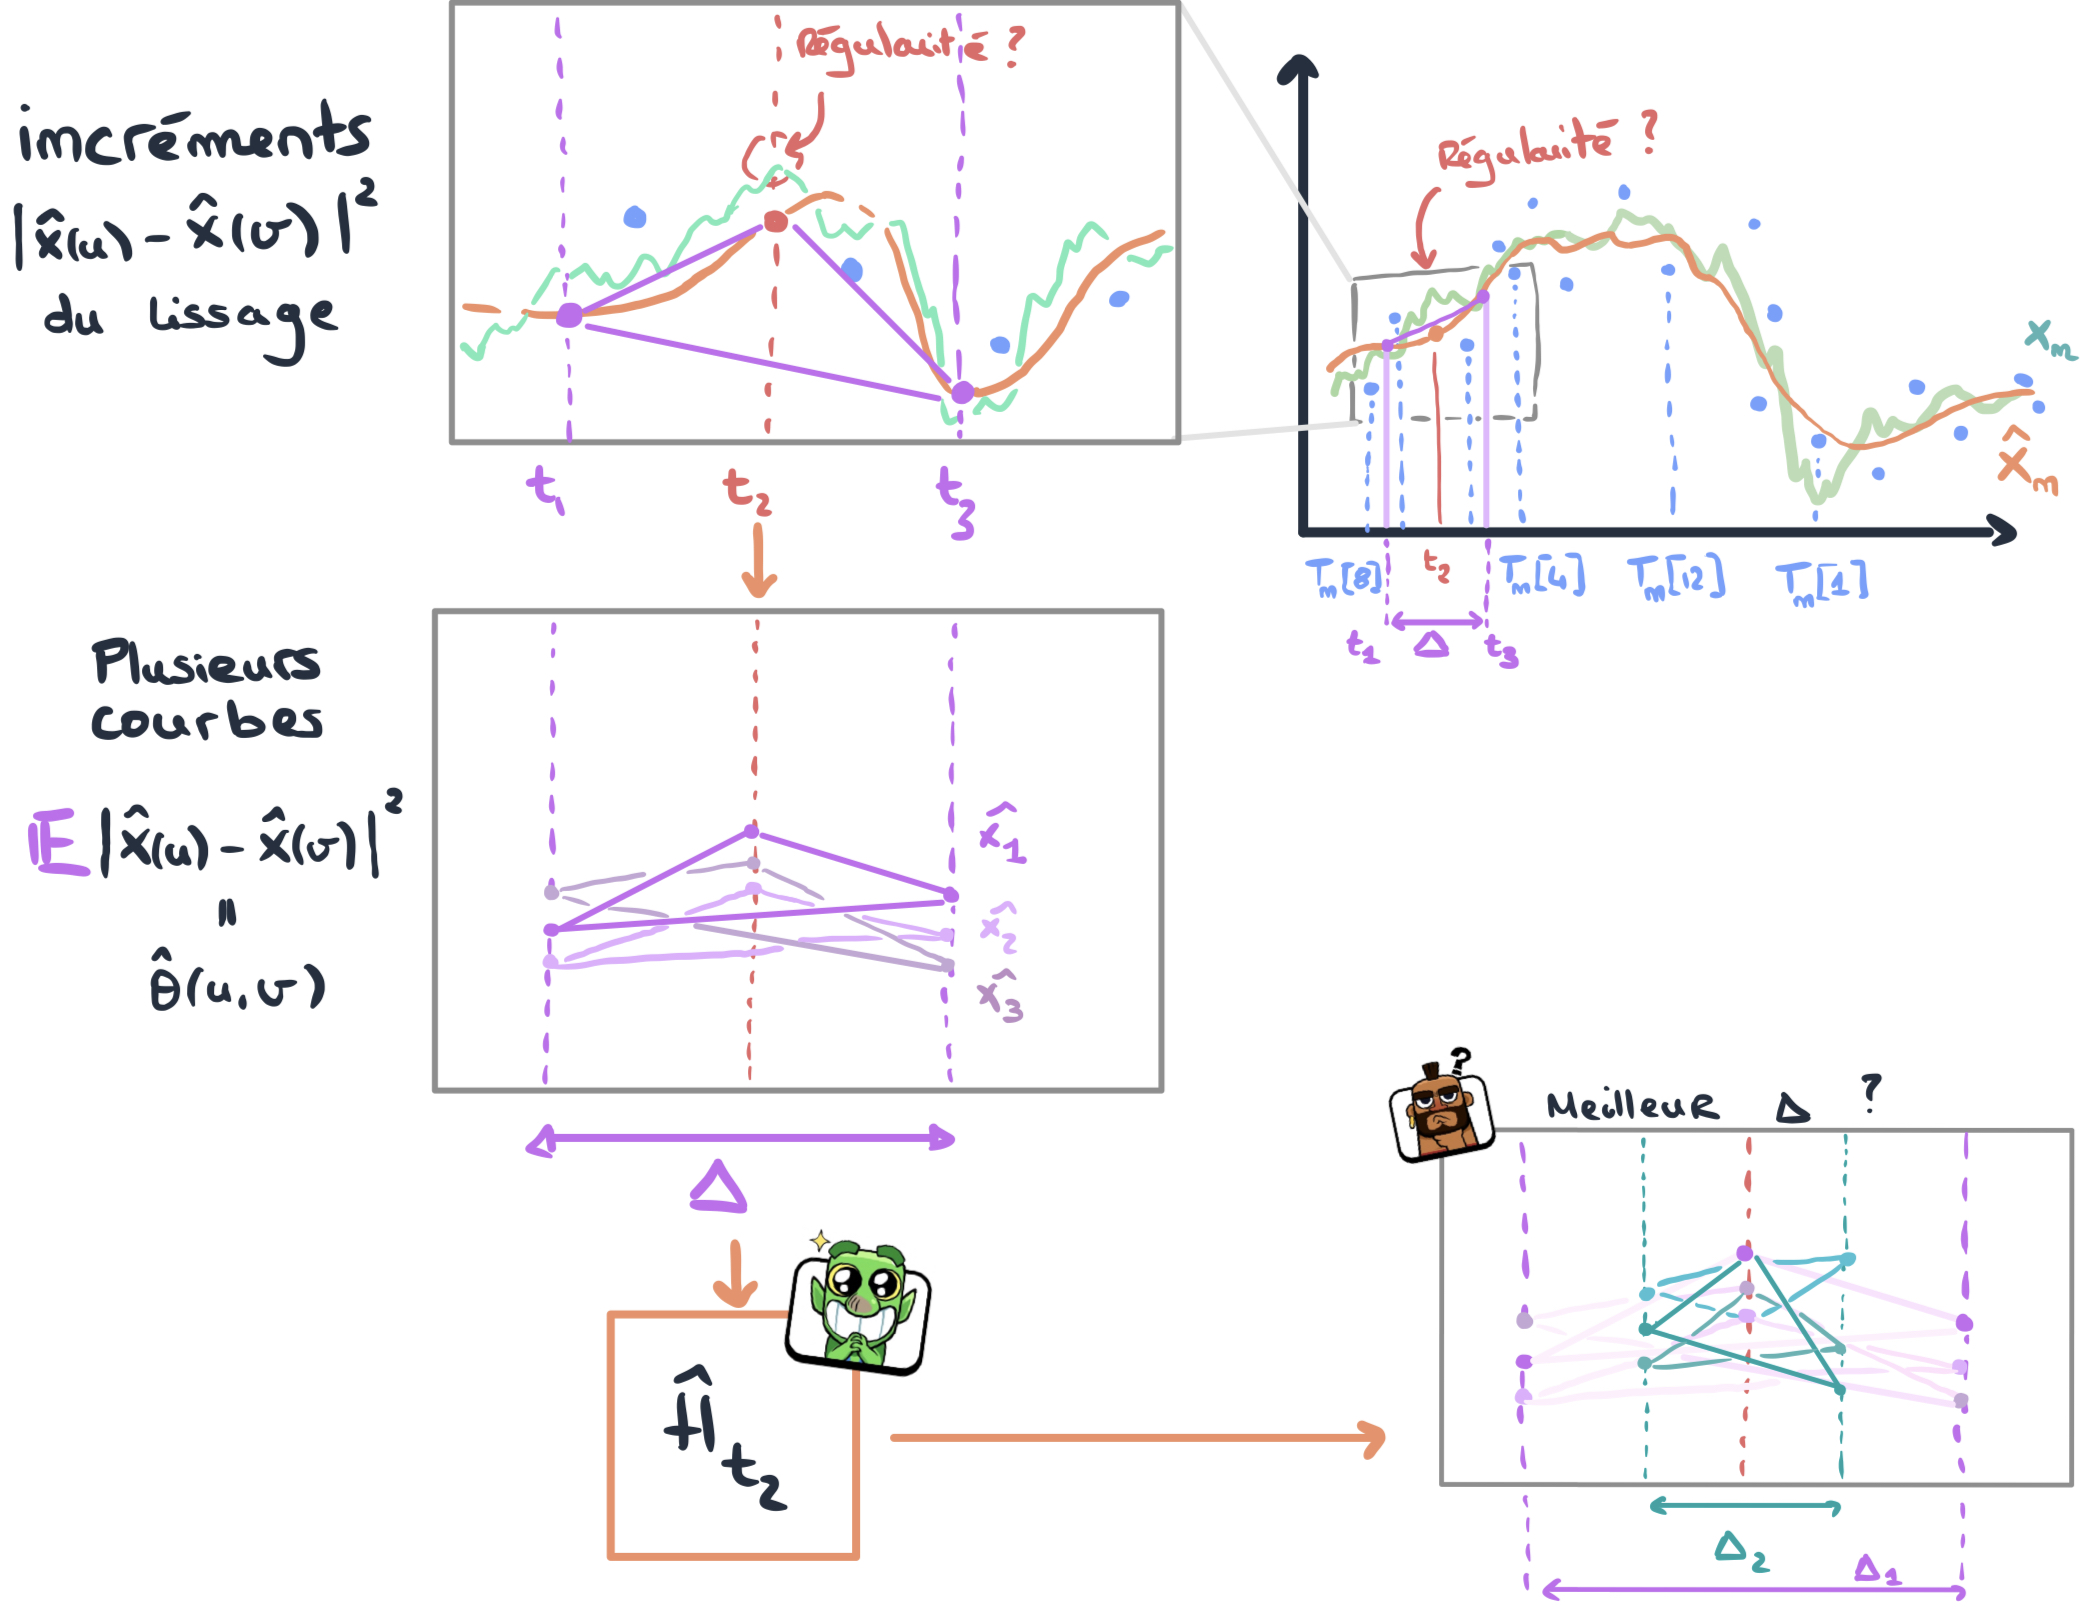
\includegraphics[width=\textwidth]{Images/sketches/estim_reg.jpg}
	\end{center}

	\caption{Schéma résumé de la méthode d'estimation de la régularité}
	\label{fig:sketch_estim_reg_methodo}
\end{figure}

\noindent La procédure d'obtention de la régularité est ainsi la suivante :

$\circled 1$ : Pré-lissage de la courbe

$\circled 2$ : Calcul des incréments quadratiques sur la courbe lissée

$\circled 3$ : moyennage des incréments (converge vers l'espérance sous hypothèse de dépendance faible)

$\circled 4$ : Utilisation de l'estimateur

Ce que nous cherchons désormais à déterminer est désormais la réponse à la question suivante :

\question{
	Quel $\Delta$ choisir pour obtenir la meilleure estimation de $H$ en $t_2$ ?
}

Pour étudier cela, nous allons simuler des données FAR(1) Höldériennes de régularité connue et allons étudier quel $\Delta$ fournit la meilleure estimation des paramètres de régularité en fonction de $\lambda$, $N$, $H_t$, ... \footnote{on pourra se référer à \ref{tab:model} pour la signification des notations}
